%% ============================================================
%% IEEE TCAD Regular Paper Template
%% --------------------------------------------------------------
%% This template targets IEEE Transactions on Computer-Aided
%% Design of Integrated Circuits and Systems (TCAD).
%%
%% Before compiling:
%%   1. Place IEEEtran.cls and IEEEtran.bst in this directory
%%      (download from https://www.ctan.org/pkg/ieeetran
%%       or copy from your existing IEEE template).
%%   2. Run: latexmk -pdf main.tex   OR   make
%%
%% Compile order if not using latexmk:
%%   pdflatex main.tex
%%   bibtex   main
%%   pdflatex main.tex
%%   pdflatex main.tex
%% ============================================================

\documentclass[journal,letterpaper]{IEEEtran}

%% ---- Math, algorithms ------------------------------------------------
\usepackage{amsmath,amsfonts,amssymb}
\usepackage{algorithm}
\usepackage{algorithmic}

%% ---- Tables & figures ------------------------------------------------
\usepackage{booktabs}
\usepackage{multirow}
\usepackage{array}
\usepackage{graphicx}
\usepackage[caption=false,font=normalsize,labelfont=sf,textfont=sf]{subfig}
\usepackage{stfloats}

%% ---- Misc -----------------------------------------------------------
\usepackage{xcolor}
\usepackage{url}
\usepackage{verbatim}
\usepackage{textcomp}
\usepackage{listings}
\usepackage{cite}                 % collapses [1,2,3,4] -> [1]-[4]
\usepackage[hidelinks]{hyperref}

%% ---- TikZ / pgfplots for vector figures -----------------------------
\usepackage{tikz}
\usepackage{pgfplots}
\pgfplotsset{compat=1.18}
\usetikzlibrary{shapes,arrows,positioning,calc,fit,backgrounds}

%% ---- Hyphenation -----------------------------------------------------
\hyphenation{op-tical net-works semi-conduc-tor}

%% ---- Revision-marking macros ----------------------------------------
%% Use \rev{...} for first-round revisions, \revtwo{...} for second-round.
%% To produce a clean (non-colored) PDF for the camera-ready, redefine
%% these macros to no-ops (see below).
\newcommand{\rev}[1]{\textcolor{blue}{#1}}
\newcommand{\revtwo}[1]{\textcolor{magenta}{#1}}
%% Camera-ready: \renewcommand{\rev}[1]{#1}\renewcommand{\revtwo}[1]{#1}

%% ---- Consistent terminology macros ----------------------------------
\newcommand{\method}{\textsc{YourMethod}}     % placeholder method name
\newcommand{\eg}{e.g.,\xspace}
\newcommand{\ie}{i.e.,\xspace}
\newcommand{\etal}{\textit{et~al.}\xspace}

%% ---- Listings for code (Verilog / Python / etc.) --------------------
\definecolor{codegreen}{rgb}{0,0.6,0}
\definecolor{codegray}{rgb}{0.5,0.5,0.5}
\definecolor{codepurple}{rgb}{0.58,0,0.82}
\definecolor{backcolour}{rgb}{0.97,0.97,0.95}
\lstset{
  backgroundcolor=\color{backcolour},
  basicstyle=\ttfamily\small,
  keywordstyle=\color{blue}\bfseries,
  commentstyle=\color{codegreen},
  stringstyle=\color{codepurple},
  numbers=left,
  numberstyle=\tiny\color{codegray},
  frame=single,
  breaklines=true,
  showstringspaces=false,
  tabsize=2,
  xleftmargin=1.5em,
  framexleftmargin=1em
}

%% ============================================================
%% Title, authors, and IEEE markings
%% ============================================================

\title{Your Paper Title: A Concise Description of the Contribution Following IEEE TCAD Conventions}

\author{First~Author,~\IEEEmembership{Member,~IEEE,}
        Second~Author,~\IEEEmembership{Senior~Member,~IEEE,}
        and~Third~Author,~\IEEEmembership{Fellow,~IEEE}%
\thanks{F.~Author and S.~Author are with the Department of Electrical and Computer Engineering, University~Name, City, State, ZIP, Country (e-mail: first.author@example.edu; second.author@example.edu).}%
\thanks{T.~Author is with the Department of Computer Science, University~Name, City, State, ZIP, Country (e-mail: third.author@example.edu).}%
\thanks{Manuscript received April 19, 2026; revised August 26, 2026.}%
\thanks{Corresponding author: First Author.}%
}

%% Page header
\markboth{IEEE Transactions on Computer-Aided Design of Integrated Circuits and Systems}%
{Author \MakeLowercase{\textit{et al.}}: Short Paper Title for Page Header}

%% ============================================================
\begin{document}

\maketitle

%% ---- Abstract -------------------------------------------------------
\begin{abstract}
% Recommended structure (200-250 words):
%  (1) Problem context (1-2 sentences). What EDA / circuit problem.
%  (2) Limitation of prior work (1 sentence). Why existing approaches fall short.
%  (3) Proposed method ("In this paper, we propose...") (1-2 sentences).
%  (4) Key technical insight or mechanism (1-2 sentences). The "how".
%  (5) Experimental evidence with concrete numbers.
%
% Avoid generic ML-style openers. State the problem concretely.

\textbf{[REPLACE]} \method{} is an open-source / industrial-grade
[algorithm / framework / methodology] for [specific EDA problem at a
specific design level]. Existing approaches [briefly: limitation].
We propose [the key idea in one or two sentences], which [the mechanism].
Experimental results on the [benchmark suite, with citation] suite, using
the [PDK / library] and the [tool flow with version], show that the
proposed method achieves [headline number 1] and [headline number 2]
compared to the strongest prior baseline [cite].
\end{abstract}

%% ---- IEEE Keywords --------------------------------------------------
\begin{IEEEkeywords}
Computer-aided design, electronic design automation, [3-5 more terms
specific to your contribution].
\end{IEEEkeywords}

%% ---- IEEE convention: ----------------------------------------------
\IEEEpeerreviewmaketitle

%% ============================================================
%% Sections (each in a separate file under content/)
%% ============================================================

\section{Introduction}
\label{sec:intro}

% Recommended structure (1.5--2 columns of IEEEtran):
%   Paragraph 1: Problem context (industry / scaling / technology trend)
%   Paragraph 2: Why prior approaches fall short
%   Paragraph 3: This work in one paragraph, leading into contribution bullets
%   Bulleted contribution list (3--5 bullets)
%   Paragraph 4: Paper roadmap

\IEEEPARstart{T}{he} continuing scaling of integrated circuits and the
increasing complexity of modern System-on-Chip (SoC) designs make
[the specific EDA problem you address] a central challenge for
chip-design productivity and quality of results (\QoR). \textbf{[REPLACE
with one to two sentences of industry / EDA flow context, with a concrete
example.]}

Prior work on this problem can be broadly grouped into [N] families.
\rev{One family of methods \cite{PLACEHOLDER_family1_a, PLACEHOLDER_family1_b}
relies on [approach], which achieves [property] but suffers from
[limitation].} A second family \cite{PLACEHOLDER_family2_a, PLACEHOLDER_family2_b}
adopts [different approach], achieving [property] but at the cost of
[other limitation]. To our knowledge, no existing method achieves all
three of \textit{[property A]}, \textit{[property B]}, and \textit{[property C]}
simultaneously.

In this paper, we propose \method{}, a [class of artifact, \eg{} algorithm,
framework, methodology] for [specific EDA problem]. \method{} combines
[ingredient 1] with [ingredient 2] in a [novel way / formulation], and is
designed to achieve [property A], [property B], and [property C]
simultaneously. We evaluate \method{} on [benchmark suites] using the
[PDK, tool flow]. Experimental results show that \method{} achieves
[headline result 1] and [headline result 2] compared to the strongest
prior baseline \cite{PLACEHOLDER_baseline}.

\textbf{Contributions.} This paper makes the following contributions:

\begin{itemize}
    \item We identify [a specific limitation of prior work] and characterize
          it on [N] benchmark designs (Section~\ref{sec:background}).
    \item We propose \method{}, a [class of method] that addresses this
          limitation by [the key idea] (Section~\ref{sec:method}).
    \item We provide [analytical / theoretical] evidence that \method{}
          [property], with complexity [\(O(n \log n)\) or similar]
          (Section~\ref{sec:method}).
    \item We evaluate \method{} on the [benchmark suite] and report
          [headline result] over [N] baselines, including [B1] and [B2]
          (Section~\ref{sec:experiments}).
    \item We release the implementation as open source at
          \texttt{[URL or anonymous mirror during review]}
          (Section~\ref{sec:experiments}).
\end{itemize}

The rest of this paper is organized as follows.
Section~\ref{sec:background} reviews relevant background and prior work.
Section~\ref{sec:method} presents \method{} in detail.
Section~\ref{sec:experiments} describes the experimental setup and
results. Section~\ref{sec:discussion} discusses limitations and threats
to validity. Section~\ref{sec:conclusion} concludes.

\section{Background and Related Work}
\label{sec:background}
\label{sec:related}

% This is ONE combined Section II. Pick ONE name for it -- "Background
% and Related Work", "Background", or "Related Work" -- and stick with it.
%
% Do NOT split this into "Background" + "Related Work" (neither as two
% peer top-level sections, NOR as two subsections named "Background" and
% "Related Work" inside this section). If you use subsections at all,
% group them BY TOPIC / APPROACH (one subsection per line of prior work),
% as illustrated below. A short paper can also be a flat section with no
% subsections.
%
% Necessary primer material (terminology, formal definitions, recap of
% prior techniques the reader must know) is woven into the relevant
% topical subsections, NOT separated into its own "Background" subsection.
%
% Reviewers prefer methodological organization (group by *approach*, not
% by *paper*). Avoid the "X et al. did A. Y et al. did B." pattern.

[REPLACE] One short opening paragraph: name the two or three research
communities your work sits between, list the topical subsections that
follow, and point forward to your comparison table if you have one.

\subsection{[Topic / Approach Group 1]}
\label{sec:bg_group1}

\textbf{[Group 1: most closely related approach.]} One line of work
formulates [problem] as [classical formulation]
\cite{PLACEHOLDER_g1_a, PLACEHOLDER_g1_b, PLACEHOLDER_g1_c}. These
methods achieve [property] but assume [assumption]. Weave in any
terminology or formal definitions the reader needs here, rather than
in a separate primer subsection. \method{} follows this line but
differs in [specific difference].

\subsection{[Topic / Approach Group 2]}
\label{sec:bg_group2}

\textbf{[Group 2: alternative approach.]} A second line of work uses
[different formulation, \eg{} ILP, gradient-based, ML-driven]
\cite{PLACEHOLDER_g2_a, PLACEHOLDER_g2_b}. These approaches achieve
[property] at the cost of [limitation]. \method{} differs in
[specific difference, with justification].

\subsection{[Topic / Approach Group 3, if applicable]}
\label{sec:bg_group3}

\textbf{[Group 3: ML / learning-based approach, if applicable.]}
Several recent works apply [deep learning / reinforcement learning / GNN]
to [problem] \cite{PLACEHOLDER_ml_a, PLACEHOLDER_ml_b}.
These methods are orthogonal to \method{} in that [reason for being
orthogonal]; combining them is left as future work.

\subsection{The Gap}
\label{sec:bg_gap}

\textbf{Distinction.} \method{} is the first method, to our knowledge,
that [claim that summarizes the gap in the literature]. The closest prior
method is \cite{PLACEHOLDER_closest}, which differs in [specific
difference]; we compare against it directly in
Section~\ref{sec:experiments}.

\section{The Proposed Method: \method{}}
\label{sec:method}

% Recommended structure (adapt to fit your contribution):
%   III.A  Overview (with Figure 1)
%   III.B  Formal problem statement / preliminaries
%   III.C  Core algorithm or framework with pseudocode
%   III.D  (Optional) Complexity / theoretical analysis
%   III.E  Implementation details (parameters, defaults)
%
% Re-section as appropriate. Not every paper needs all of these
% subsections; not every paper has a multi-stage pipeline.

\subsection{Overview}
\label{sec:method:overview}

Figure~\ref{fig:overview} shows the high-level structure of \method{}.
\textbf{[REPLACE with a 2--3 sentence summary of the framework and where
the novelty lies. Adapt the figure below to match.]}

\begin{figure}[!t]
    \centering
    % Placeholder TikZ overview diagram.
    % Replace with your real figure (TikZ preferred over raster).
    \begin{tikzpicture}[
        node distance=0.6cm,
        block/.style={draw, rectangle, rounded corners=2pt,
                      minimum width=2.2cm, minimum height=0.7cm,
                      align=center, font=\small},
        arrow/.style={-Stealth, thick}
    ]
        \node[block, fill=blue!10]   (in)   {Input\\(\eg{} RTL or netlist)};
        \node[block, right=of in, fill=green!10]  (s1) {Stage 1};
        \node[block, right=of s1, fill=orange!10] (s2) {Stage 2\\(novel)};
        \node[block, right=of s2, fill=red!10]    (s3) {Stage 3};
        \node[block, right=of s3]                  (out){Output\\(\eg{} placed design)};
        \draw[arrow] (in)--(s1);
        \draw[arrow] (s1)--(s2);
        \draw[arrow] (s2)--(s3);
        \draw[arrow] (s3)--(out);
    \end{tikzpicture}
    \caption{Overview of \method{}. Stages~1 and~3 follow standard EDA
    practice; Stage~2 (highlighted) is the novel component proposed in
    this paper, described in Section~\ref{sec:method:core}.}
    \label{fig:overview}
\end{figure}

\subsection{Preliminaries and Notation}
\label{sec:method:prelim}

\textbf{[REPLACE]} We adopt the following notation throughout the paper.
Let \(D\) denote a [design / netlist / placement instance] with [N] cells
and [M] nets. The objective is to minimize
\(\Phi(D) = \alpha \cdot \mathrm{area}(D) + \beta \cdot \mathrm{delay}(D)
+ \gamma \cdot \mathrm{power}(D)\), subject to [constraints]. The
hyperparameters \(\alpha, \beta, \gamma\) are set in
Section~\ref{sec:method:impl}.

\subsection{Core Algorithm}
\label{sec:method:core}

The core of \method{} is summarized in Algorithm~\ref{alg:method}.

\begin{algorithm}[!t]
\caption{\method{}: high-level procedure.}
\label{alg:method}
\begin{algorithmic}[1]
\REQUIRE Design \(D\), parameters \(\theta = (\alpha,\beta,\gamma)\)
\ENSURE Optimized design \(D^*\)
\STATE \(D_0 \leftarrow \text{Stage1}(D)\)
\STATE \(k \leftarrow 0\); \(\Phi_{\text{prev}} \leftarrow \infty\)
\WHILE{not converged}
    \STATE \(D_{k+1} \leftarrow \text{Stage2}(D_k, \theta)\)
        \COMMENT{novel step (Sec.~\ref{sec:method:core})}
    \STATE \(\Phi_k \leftarrow \Phi(D_{k+1})\)
    \IF{\(|\Phi_{\text{prev}} - \Phi_k| < \varepsilon\)}
        \STATE \textbf{break}
    \ENDIF
    \STATE \(\Phi_{\text{prev}} \leftarrow \Phi_k\); \(k \leftarrow k+1\)
\ENDWHILE
\STATE \(D^* \leftarrow \text{Stage3}(D_{k+1})\)
\RETURN \(D^*\)
\end{algorithmic}
\end{algorithm}

\textbf{Stage 1 — [REPLACE name].} [Two-three sentences explaining the
stage. Cite related work used at this stage.]

\textbf{Stage 2 — [REPLACE name, the novel part].} The key insight is
that [the insight]. We formalize this as follows:

\begin{equation}
\label{eq:novel}
f(D) \;=\; \sum_{e \in E} w(e) \cdot \phi\!\left(\, x(e) \,\right)
       \;+\; \lambda \, R(D),
\end{equation}

\noindent where \(w(\cdot)\) is the [weight function], \(\phi(\cdot)\) is
[smoothing function], and \(R(\cdot)\) is the [regularization term]
weighted by \(\lambda\). The function \(f(D)\) is solved by [optimization
method, \eg{} L-BFGS / coordinate descent / dynamic programming], yielding
[output property].

\textbf{Stage 3 — [REPLACE name].} [Two-three sentences.]

\subsection{Complexity Analysis}
\label{sec:method:complexity}

\textbf{[REPLACE]} The dominant cost of Algorithm~\ref{alg:method} is
Stage~2, which performs \(O(\log(1/\varepsilon))\) iterations of
\(O(n \log n)\) work each, where \(n\) is the number of cells in the
design and \(\varepsilon\) is the convergence tolerance. Total time
complexity is therefore \(O(n \log n \cdot \log(1/\varepsilon))\).
Memory usage is \(O(n + m)\) where \(m\) is the number of nets.
We empirically validate this scaling in
Section~\ref{sec:experiments:scaling}.

\subsection{Implementation Details}
\label{sec:method:impl}

\textbf{[REPLACE]} \method{} is implemented in approximately [N] lines of
[Python / C++] on top of [base tool, \eg{} OpenROAD]. The default
hyperparameters are \(\alpha = 1.0\), \(\beta = 0.5\), \(\gamma = 0.1\),
and \(\varepsilon = 10^{-3}\); these were tuned on the validation subset
described in Section~\ref{sec:experiments:setup} and held fixed across
all reported experiments. The convergence tolerance \(\varepsilon\)
typically triggers in 8--12 outer iterations on designs we tested.

\section{Experimental Evaluation}
\label{sec:experiments}

\subsection{Experimental Setup}
\label{sec:experiments:setup}

% State the setup at the level of detail your sub-community expects for
% reproducibility. Replace each bracketed item with what is relevant in
% your sub-area (tool versions, datasets / benchmarks, hardware, etc.).

\textbf{Platform.} All experiments were performed on \textbf{[REPLACE
with hardware: CPU/GPU model, RAM, OS]}.

\textbf{Implementation.} \method{} is implemented in approximately
\textbf{[N]} lines of \textbf{[language]}, building on
\textbf{[base toolchain or libraries]}. \textbf{[Add tool versions /
commit hashes as appropriate for reproducibility.]}

\textbf{Datasets / Benchmarks.} We evaluate on \textbf{[REPLACE: the
benchmark suite(s) used, with citations]}. The benchmarks span
\textbf{[characterize: scope, size range, design family, etc.]}.

\textbf{Baselines.} We compare against the following baselines, each
re-run under identical conditions where possible to ensure a fair
comparison:
\begin{itemize}
    \item \textbf{Baseline 1} \cite{PLACEHOLDER_baseline1} -- a
          representative method of [class of approach].
    \item \textbf{Baseline 2} \cite{PLACEHOLDER_baseline2} -- the
          current best published result on these benchmarks.
    \item \textbf{[Optional]} For baselines without publicly available
          implementations, we cite numbers from the original papers and
          note this in the relevant tables.
\end{itemize}

\textbf{Metrics.} We report \textbf{[REPLACE with the metrics relevant
to your contribution]}. \textbf{[If multiple metrics matter for your
sub-community, list them all; for each metric, state the direction
(higher is better / lower is better) and the units.]}

\textbf{Reporting.} Each value is the average of \textbf{[K]} runs with
different random seeds. We report standard deviation for any metric
where the run-to-run variance exceeds 1\% of the mean.

\subsection{Main Results}
\label{sec:experiments:main}

Table~\ref{tab:main} reports the main results of \method{} compared to
the baselines. \textbf{[REPLACE with your concrete observations.]}
\method{} achieves \textbf{[headline result 1]} and \textbf{[headline
result 2]} compared to the strongest baseline
\cite{PLACEHOLDER_baseline2}.

\begin{table*}[!t]
\caption{Main Comparison Against Baselines. Bold marks the best value per row.}
\label{tab:main}
\centering
\small
\begin{tabular}{l|cc|cc|cc}
\toprule
 & \multicolumn{2}{c|}{Baseline 1 \cite{PLACEHOLDER_baseline1}}
 & \multicolumn{2}{c|}{Baseline 2 \cite{PLACEHOLDER_baseline2}}
 & \multicolumn{2}{c}{\textbf{\method{} (Ours)}} \\
Design / Setting & Metric 1 & Metric 2 & Metric 1 & Metric 2 & Metric 1 & Metric 2 \\
\midrule
[design / setting 1] & --- & --- & --- & --- & --- & --- \\
[design / setting 2] & --- & --- & --- & --- & --- & --- \\
\midrule
Average / Geo. Mean & --- & --- & --- & --- & \textbf{---} & \textbf{---} \\
\bottomrule
\end{tabular}
\end{table*}

\subsection{Ablation Study}
\label{sec:experiments:ablation}

\textbf{[REPLACE]} To isolate the contribution of each component of
\method{}, we report an ablation in Table~\ref{tab:ablation}. Disabling
\textbf{[the novel stage]} degrades \textbf{[metric]} by
\textbf{[X\%]}, while disabling \textbf{[other component]} degrades
\textbf{[metric]} by \textbf{[Y\%]}. This confirms that both components
of \method{} contribute materially to the observed improvement.

\begin{table}[!t]
\caption{Ablation Study: Effect of Disabling Each Component of \method{}.}
\label{tab:ablation}
\centering
\small
\begin{tabular}{lcc}
\toprule
Configuration & Metric 1 & Metric 2 \\
\midrule
Full \method{} (Ours)             & --- & --- \\
~~w/o component A                 & --- & --- \\
~~w/o component B                 & --- & --- \\
~~w/o iterative refinement        & --- & --- \\
\bottomrule
\end{tabular}
\end{table}

\subsection{Scaling and Runtime}
\label{sec:experiments:scaling}

\textbf{[Optional --- include only if scaling is relevant to your
contribution.]} Figure~\ref{fig:scaling} shows the runtime of \method{}
as a function of \textbf{[input size variable]}. The observed scaling is
consistent with the \textbf{[\(O(n \log n)\) or similar]} analysis in
Section~\ref{sec:method:complexity}.

\begin{figure}[!t]
    \centering
    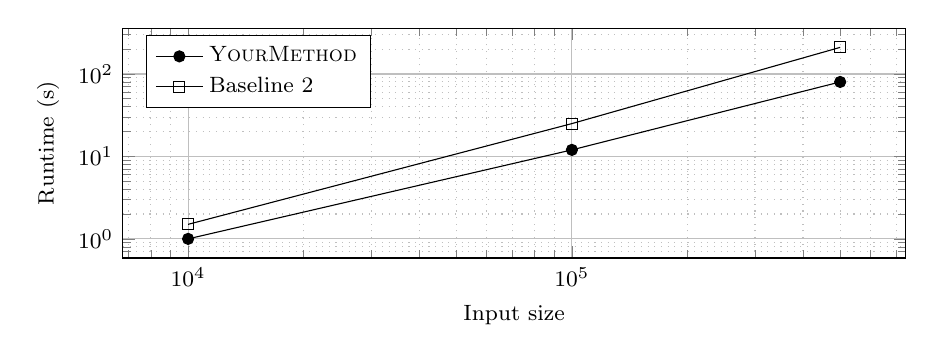
\begin{tikzpicture}
        \begin{loglogaxis}[
            width=0.95\columnwidth, height=4.5cm,
            xlabel={Input size},
            ylabel={Runtime (s)},
            grid=both, minor grid style={dotted},
            legend pos=north west, legend cell align=left,
            font=\footnotesize
        ]
        \addplot[mark=*]      coordinates {(1e4,1.0)(1e5,12)(5e5,80)};
        \addlegendentry{\method{}}
        \addplot[mark=square] coordinates {(1e4,1.5)(1e5,25)(5e5,210)};
        \addlegendentry{Baseline 2}
        \end{loglogaxis}
    \end{tikzpicture}
    \caption{Runtime scaling of \method{}. \method{} scales approximately
    as \(O(n \log n)\), consistent with Section~\ref{sec:method:complexity}.}
    \label{fig:scaling}
\end{figure}

\subsection{Sensitivity to Hyperparameters}
\label{sec:experiments:sensitivity}

\textbf{[Optional --- include if your method has hyperparameters whose
sensitivity matters.]} We sweep the regularization weight \(\lambda\)
from \(10^{-3}\) to \(10^{1}\). \method{} is stable across two orders
of magnitude, with the best results at \(\lambda = \textbf{[value]}\).
The full sweep is reported in the supplementary material.

\subsection{Case Study}
\label{sec:experiments:case}

\textbf{[Optional but recommended for journals --- pick one concrete,
realistic instance and walk through it in depth.]} We present a case
study on \textbf{[specific design / problem instance]} to demonstrate
the practical applicability of \method{}. Compared to the default
baseline, \method{} \textbf{[concrete improvement on this instance]}.

\section{Discussion}
\label{sec:discussion}

\subsection{Limitations and Threats to Validity}
\label{sec:discussion:limitations}

% TCAD does not require a "Limitations" section, but reviewers respect
% honest discussion. Include this if you have space.

\textbf{[REPLACE]} While \method{} consistently improves [metric] on the
benchmarks evaluated, several limitations are worth noting.

\textbf{Coverage of benchmarks / settings.} Our evaluation covers
\textbf{[the scope you evaluated]}. We have not evaluated on
\textbf{[settings out of scope --- if any]}. We expect \method{} to
generalize but cannot make formal guarantees beyond the evaluated
regime.

\textbf{Hyperparameter sensitivity.} The default hyperparameters were
selected on a validation subset (Section~\ref{sec:experiments:setup}).
Instances with extreme characteristics may require re-tuning, as
discussed in Section~\ref{sec:experiments:sensitivity}.

\textbf{Comparison to closed-source / proprietary baselines.} We compare
against \textbf{[the publicly accessible baselines you used]}, but
\textbf{[any closed-source / commercial alternative you could not
re-run]} is out of reach due to \textbf{[licensing / availability
reasons]}. Direct comparison against such tools is left for future work.

\subsection{Future Work}
\label{sec:discussion:future}

Future work will explore:
(i) \textbf{[direction 1]};
(ii) \textbf{[direction 2]};
(iii) \textbf{[direction 3]}.

\section{Conclusion}
\label{sec:conclusion}

% Two paragraphs maximum. Restate contribution + headline numbers + brief
% forward look.

\textbf{[REPLACE]} We presented \method{}, a [class of method] for
[specific EDA problem at a specific design level]. The key idea is
[one-sentence summary]. Across [N] benchmark designs from the EPFL and
ITC'99 suites, \method{} reduces [metric A] by [X\%] and [metric B] by
[Y\%] compared to the strongest open-source baseline, while maintaining
[other metric].

By making [specific aspect] explicitly addressable, \method{} aims to
unblock [downstream tooling improvement] in the EDA flow. The implementation
is released as open source at
\texttt{[URL or anonymous mirror during review]}, and we hope it serves
as a useful building block for subsequent research on
[broader research direction].


%% ============================================================
%% Acknowledgments (optional; for camera-ready)
%% ============================================================
\section*{Acknowledgments}
The authors would like to thank [funding source(s)] for supporting this
work, and [collaborators / reviewers] for valuable feedback. % REPLACE

%% ============================================================
%% Bibliography
%% ============================================================
\bibliographystyle{IEEEtran}
\bibliography{refs}

%% ============================================================
%% Author biographies (camera-ready only; comment out during review)
%% ============================================================
% \begin{IEEEbiography}[{\includegraphics[width=1in,height=1.25in,clip,keepaspectratio]{figs/bio_first.jpg}}]{First Author}
% (M'18) received the B.S. and Ph.D. degrees in Electrical Engineering from
% [University], in [Year]. He is currently an [Position] at [Affiliation].
% His research interests include [topics]. He is a member of the IEEE.
% \end{IEEEbiography}

% \begin{IEEEbiographynophoto}{Second Author}
% biography text without a photo
% \end{IEEEbiographynophoto}

\end{document}
